\documentclass[12pt,a4paper]{article}

\usepackage[provide=*,polish]{babel}
\usepackage[T1]{fontenc}
\usepackage[utf8]{inputenc}
\usepackage{lmodern}
\usepackage{geometry}
\usepackage{setspace}
\usepackage{amsmath}
\usepackage{amssymb}
\usepackage{booktabs}
\usepackage{graphicx}

\geometry{margin=2.2cm}
\setstretch{1.15}
\emergencystretch=2em
\graphicspath{{figures/}}

\begin{document}

\section{Skalowanie reakcji względem liczby wyświetleń}

\textbf{Pytanie badawcze:} Czy wraz ze wzrostem liczby wyświetleń polubienia, komentarze i udostępnienia rosły proporcjonalnie, czy poszczególne rodzaje reakcji zachowywały się inaczej?

Analiza obejmuje $103$ filmy. Dla każdego z nich wykorzystano liczbę wyświetleń oraz trzy podstawowe rodzaje reakcji: polubienia, komentarze i udostępnienia. Dodatkowo utworzono zmienną obejmującą aktywne reakcje:

\[
A_i=C_i+S_i,
\]

gdzie $C_i$ oznacza liczbę komentarzy, a $S_i$ liczbę udostępnień $i$-tego filmu. Polubienie traktujemy jako najprostszą reakcję na materiał, natomiast komentarz i udostępnienie wymagają od odbiorcy większego zaangażowania. Nie analizujemy jednak komentarzy i udostępnień wyłącznie przez ich sumę. Są to różne zachowania, dlatego najpierw badamy je osobno, a połączony wskaźnik traktujemy jako wynik uzupełniający.

\subsection{Model skalowania}

Dla każdego rodzaju reakcji oszacowano osobny model log--log:

\[
\ln(Y_i)=\alpha+\gamma\ln(V_i)+\varepsilon_i,
\]

gdzie:

\begin{itemize}
    \item $Y_i$ oznacza liczbę danego rodzaju reakcji dla $i$-tego filmu
    \item $V_i$ oznacza liczbę wyświetleń filmu
    \item $\alpha$ jest wyrazem wolnym
    \item $\gamma$ jest elastycznością reakcji względem liczby wyświetleń
    \item $\varepsilon_i$ obejmuje różnice między filmami, których nie opisuje sam zasięg
\end{itemize}

Po przekształceniu model ma postać:

\[
Y_i=e^{\alpha}V_i^{\gamma}e^{\varepsilon_i}.
\]

Pomijając składnik losowy, możemy więc zapisać:

\[
Y\approx cV^{\gamma},
\qquad
c=e^{\alpha}.
\]

Parametr $\gamma$ pokazuje, jak szybko rośnie liczba reakcji w stosunku do liczby wyświetleń. Jego interpretacja zależy od położenia względem wartości $1$:

\begin{itemize}
    \item $\gamma<1$ oznacza wzrost mniej niż proporcjonalny --- reakcje rosną wolniej niż wyświetlenia, dlatego ich wskaźnik spada
    \item $\gamma=1$ oznacza wzrost proporcjonalny --- podwojeniu wyświetleń odpowiada podwojenie reakcji, a ich wskaźnik pozostaje stały
    \item $\gamma>1$ oznacza wzrost więcej niż proporcjonalny --- reakcje rosną szybciej niż wyświetlenia, dlatego ich wskaźnik wzrasta
\end{itemize}

Jeżeli przez $R$ oznaczymy wskaźnik danego rodzaju reakcji, to:

\[
R=\frac{Y}{V}.
\]

Po podstawieniu modelu potęgowego otrzymujemy:

\[
R\approx cV^{\gamma-1}.
\]

To właśnie wykładnik $\gamma-1$ opisuje zmianę wskaźnika reakcji. Dla polubień zachodzi więc bezpośredni związek z wcześniejszym modelem Like Rate:

\[
\beta_{\mathrm{Like\ Rate}}=\gamma_{\mathrm{Likes}}-1.
\]

W poprzedniej analizie otrzymano $\widehat{\beta}=-0{,}2139$. Tutaj dla liczby polubień otrzymujemy $\widehat{\gamma}=0{,}7860$, a więc:

\[
0{,}7860-1=-0{,}2140.
\]

Różnica na ostatnim miejscu po przecinku wynika z tego, że w poprzedniej analizie Like Rate był zaokrąglany do czterech miejsc po przecinku, natomiast tutaj model korzysta bezpośrednio z liczby polubień.

\subsection{Zmiana reakcji i zmiana wskaźnika}

Jeżeli liczba wyświetleń wzrasta $k$-krotnie, względną zmianę liczby reakcji obliczamy ze wzoru:

\[
100\left(k^{\widehat{\gamma}}-1\right)\%.
\]

Zmiana odpowiadającego jej wskaźnika wynosi natomiast:

\[
100\left(k^{\widehat{\gamma}-1}-1\right)\%.
\]

Są to zmiany względne, a nie zmiany wyrażone w punktach procentowych. Jeżeli przykładowo wskaźnik wynosił $5\%$ i spadł względnie o $10\%$, jego nowa wartość wynosi:

\[
5\%\cdot(1-0{,}10)=4{,}5\%.
\]

\subsection{Hipoteza o proporcjonalnym skalowaniu}

W tej analizie najważniejsza nie jest standardowa hipoteza $\gamma=0$. Wiadomo, że filmy z większą liczbą wyświetleń mają zazwyczaj również więcej reakcji. Interesuje nas to, czy reakcje rosną dokładnie w takim samym tempie jak wyświetlenia. Dla każdego modelu sprawdzamy więc:

\[
H_0:\gamma=1,
\qquad
H_1:\gamma\neq 1.
\]

Statystyka testowa ma postać:

\[
t=
\frac{\widehat{\gamma}-1}
{\operatorname{SE}_{\mathrm{HC3}}(\widehat{\gamma})}.
\]

Zastosowano odporne błędy standardowe HC3, ponieważ rozrzut reakcji nie musi być taki sam dla filmów o małym i dużym zasięgu. Jeżeli przedział ufności dla $\gamma$ obejmuje wartość $1$, dane nie dają podstaw do odrzucenia proporcjonalnego skalowania. Jeżeli cały przedział leży poniżej $1$, wskaźnik reakcji spada wraz ze wzrostem zasięgu.

\section{Wyniki w pełnej próbie}

\begin{figure}[htbp]
    \centering
    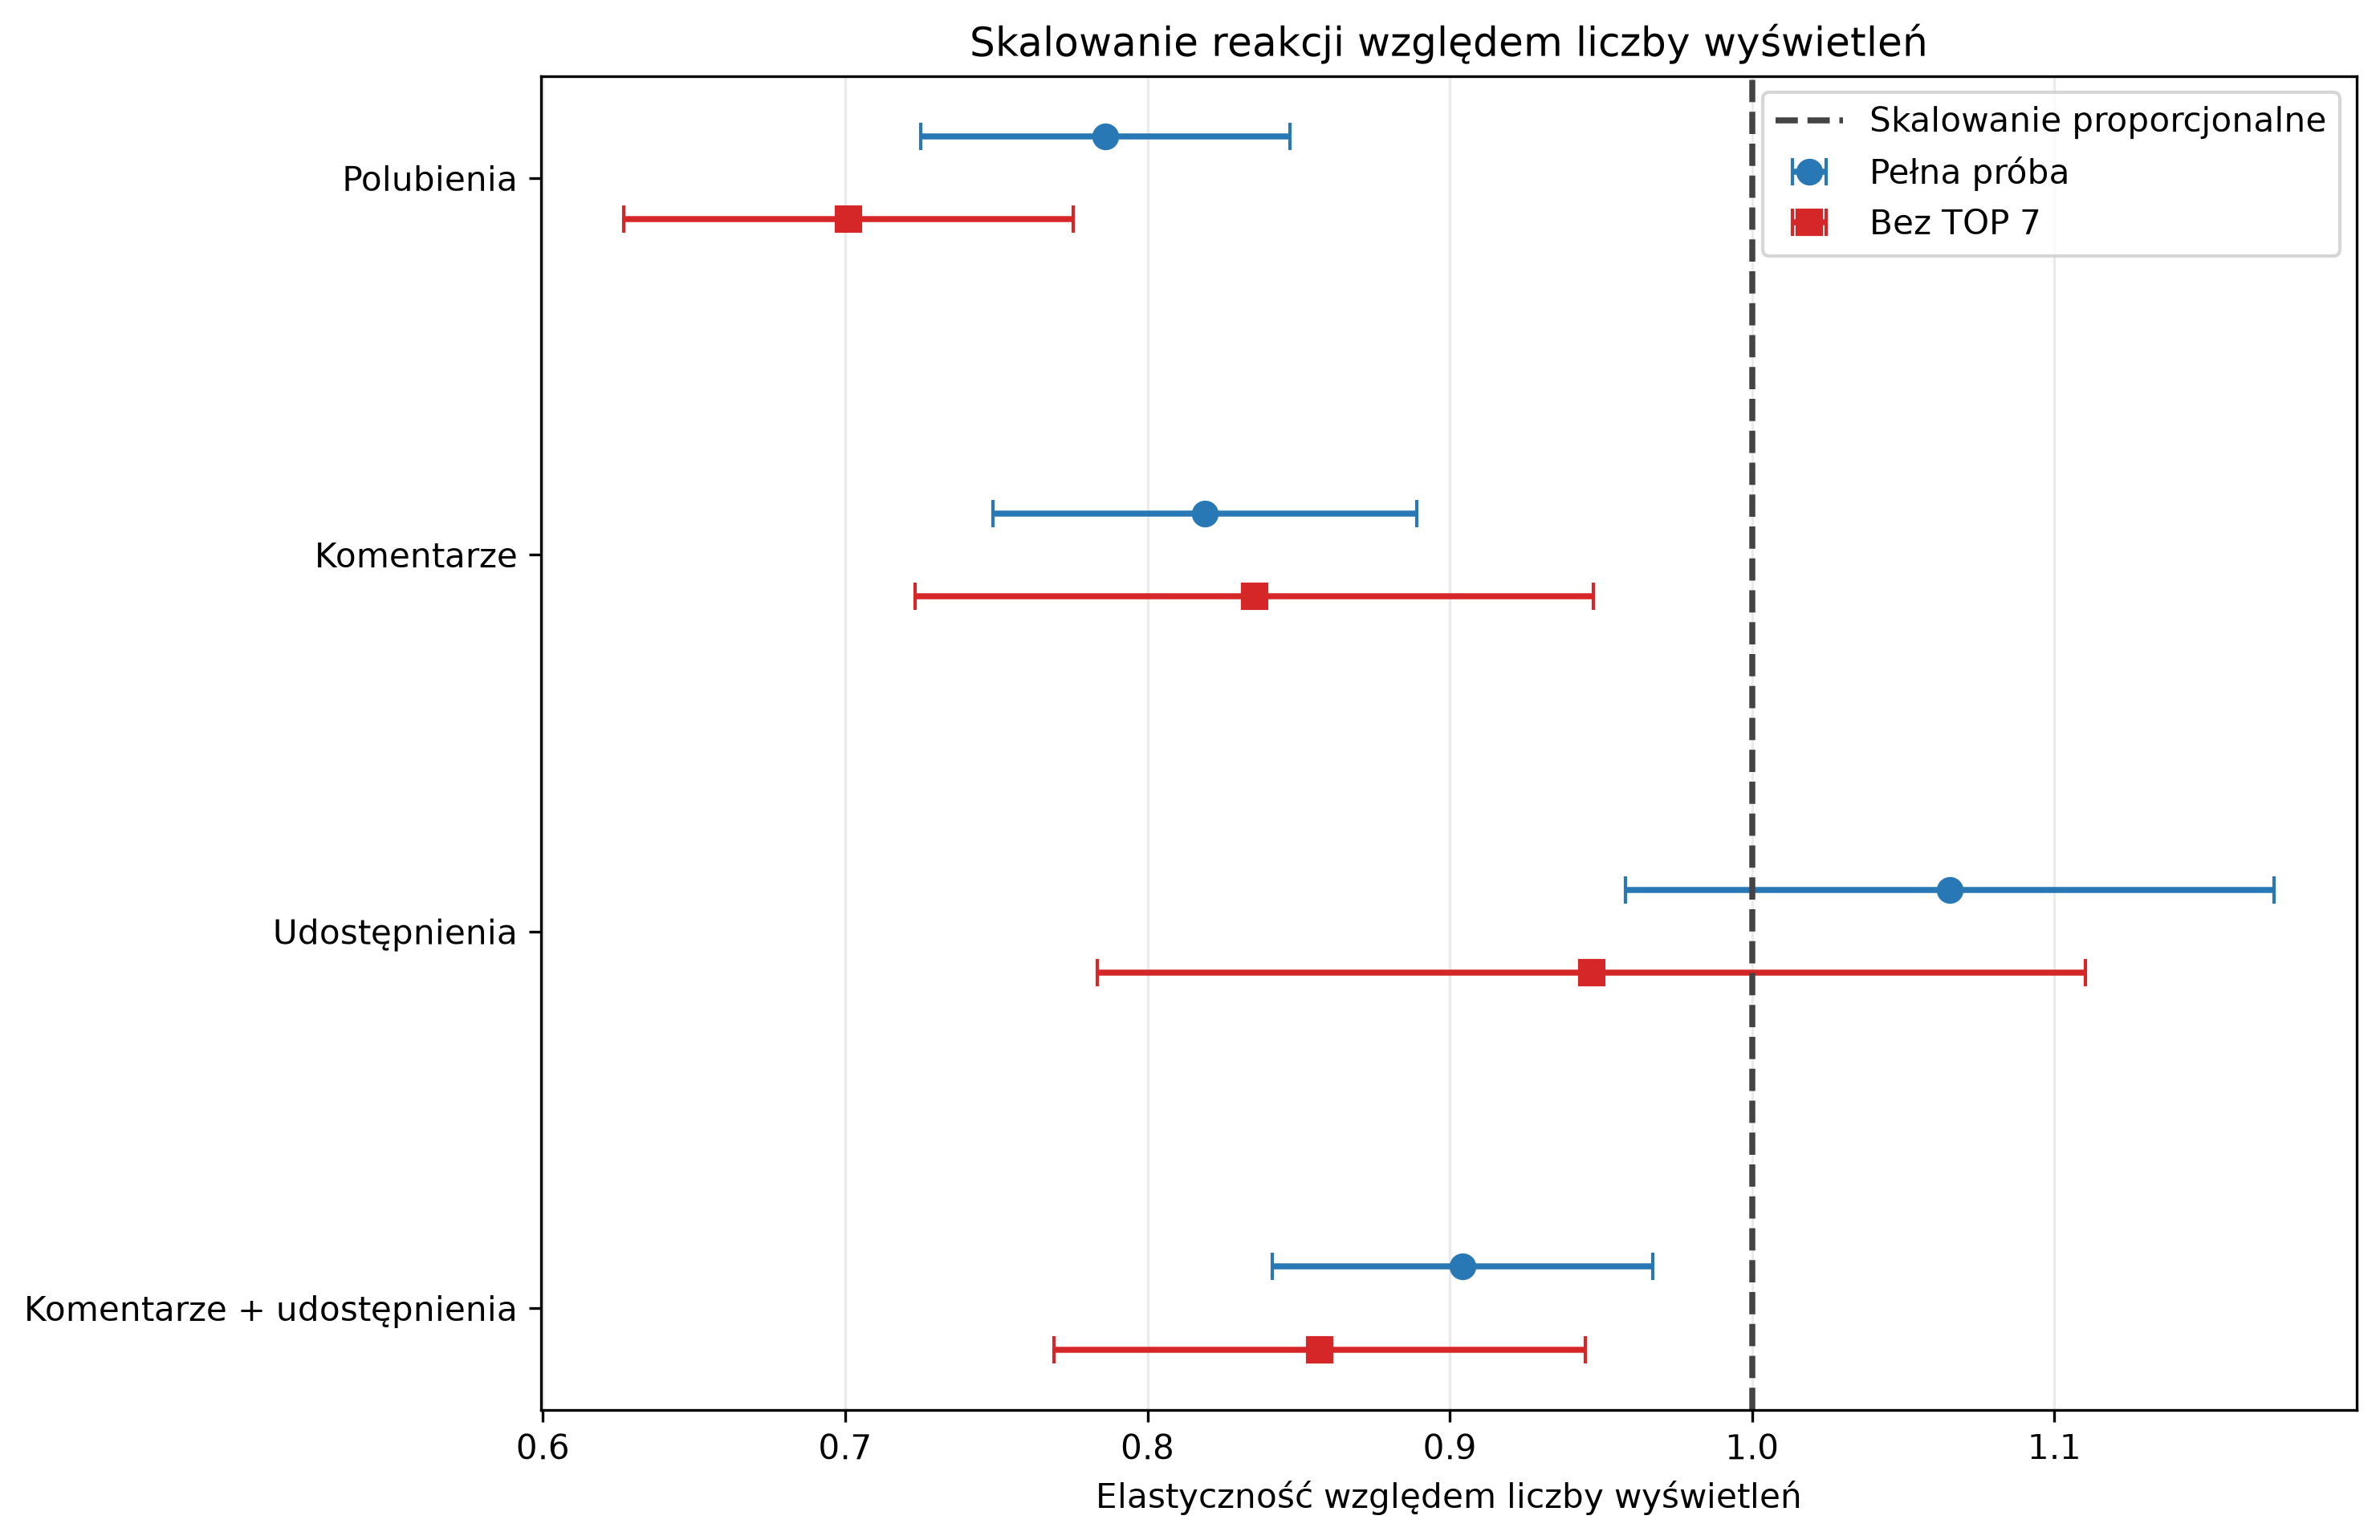
\includegraphics[width=\textwidth]{reaction_elasticities.png}
    \caption{Elastyczności reakcji w pełnej próbie i po wyłączeniu TOP 7. Przerywana linia oznacza skalowanie proporcjonalne, czyli $\gamma=1$}
    \label{fig:reaction-elasticities}
\end{figure}

Na wykresie każda kropka lub kwadrat oznacza oszacowaną elastyczność, a poziomy odcinek przedstawia $95\%$ przedział ufności. Niebieskie wyniki dotyczą pełnej próby, natomiast czerwone --- analizy bez siedmiu filmów o największej liczbie wyświetleń. Położenie całego przedziału po lewej stronie przerywanej linii oznacza, że dany rodzaj reakcji rósł wolniej niż liczba wyświetleń.

W pełnej próbie otrzymano:

\begin{center}
\small
\begin{tabular}{lcccc}
\toprule
Reakcja & $\widehat{\gamma}$ & $95\%$ CI & $p$ dla $\gamma=1$ & $R^2$ \\
\midrule
Polubienia & $0{,}7860$ & $[0{,}7249;\ 0{,}8470]$ & $3{,}5637\cdot10^{-10}$ & $0{,}9105$ \\
Komentarze & $0{,}8190$ & $[0{,}7489;\ 0{,}8891]$ & $1{,}4599\cdot10^{-6}$ & $0{,}8210$ \\
Udostępnienia & $1{,}0654$ & $[0{,}9581;\ 1{,}1727]$ & $0{,}2292$ & $0{,}7771$ \\
Komentarze $+$ udostępnienia & $0{,}9043$ & $[0{,}8414;\ 0{,}9673]$ & $0{,}0032$ & $0{,}8644$ \\
\bottomrule
\end{tabular}
\end{center}

Wartość $R^2$ odnosi się do zróżnicowania logarytmu liczby reakcji wyjaśnianego przez logarytm liczby wyświetleń. Wysokie wartości nie oznaczają, że znamy przyczyny popularności filmu. Pokazują jedynie, że zasięg jest silnie związany z bezwzględną liczbą reakcji.

\subsection{Polubienia}

Dla polubień oszacowano:

\[
\widehat{\gamma}_{L}=0{,}7860,
\qquad
95\%\ \mathrm{CI}=[0{,}7249;\ 0{,}8470].
\]

Cały przedział znajduje się poniżej $1$, a wartość $p$ dla testu proporcjonalnego skalowania wynosi $3{,}5637\cdot10^{-10}$. Liczba polubień rosła więc wyraźnie wolniej niż liczba wyświetleń.

Wzrost wyświetleń o $10\%$ wiązał się przeciętnie ze wzrostem liczby polubień o około $7{,}78\%$. Ponieważ polubienia rosły wolniej niż zasięg, Like Rate spadał wtedy względnie o około $2{,}02\%$.

Przy podwojeniu liczby wyświetleń model przewiduje:

\[
100\left(2^{0{,}7860}-1\right)\%\approx72{,}42\%
\]

więcej polubień, natomiast względna zmiana Like Rate wynosi:

\[
100\left(2^{0{,}7860-1}-1\right)\%\approx-13{,}79\%.
\]

Zasięg rośnie więc dwukrotnie, ale liczba polubień nie podwaja się. Jest to ten sam mechanizm, który w poprzedniej analizie był widoczny jako spadek Like Rate.

\subsection{Komentarze}

Dla komentarzy otrzymano:

\[
\widehat{\gamma}_{C}=0{,}8190,
\qquad
95\%\ \mathrm{CI}=[0{,}7489;\ 0{,}8891].
\]

Wynik również wskazuje na skalowanie mniej niż proporcjonalne. Przy wzroście wyświetleń o $10\%$ liczba komentarzy rosła przeciętnie o około $8{,}12\%$, a Comment Rate spadał względnie o około $1{,}71\%$.

Podwojenie liczby wyświetleń wiązało się przeciętnie ze wzrostem liczby komentarzy o około $76{,}42\%$ oraz spadkiem Comment Rate o około $11{,}79\%$.

\subsection{Udostępnienia}

Dla udostępnień otrzymano:

\[
\widehat{\gamma}_{S}=1{,}0654,
\qquad
95\%\ \mathrm{CI}=[0{,}9581;\ 1{,}1727].
\]

Punktowe oszacowanie znajduje się powyżej $1$. Wzrost wyświetleń o $10\%$ wiązał się ze wzrostem liczby udostępnień o około $10{,}69\%$, a podwojenie wyświetleń --- ze wzrostem o około $109{,}28\%$.

Nie należy jednak stwierdzać, że Share Rate na pewno wzrastał. Przedział ufności obejmuje $1$, a w teście proporcjonalnego skalowania otrzymano:

\[
p=0{,}2292.
\]

Dane są więc zgodne z sytuacją, w której liczba udostępnień rośnie w przybliżeniu proporcjonalnie do liczby wyświetleń. Szacowana zmiana Share Rate przy podwojeniu wyświetleń wynosi $+4{,}64\%$, ale nie różni się jednoznacznie od zera.

\subsection{Komentarze i udostępnienia łącznie}

Dla sumy komentarzy i udostępnień otrzymano:

\[
\widehat{\gamma}_{A}=0{,}9043,
\qquad
95\%\ \mathrm{CI}=[0{,}8414;\ 0{,}9673].
\]

Podwojenie wyświetleń wiązało się przeciętnie ze wzrostem liczby aktywnych reakcji o około $87{,}17\%$ i spadkiem Active Reaction Rate o około $6{,}42\%$. Wspólny wskaźnik spada więc znacznie łagodniej niż Like Rate, ale ukrywa różnicę między komentarzami a udostępnieniami. Właśnie dlatego osobne modele są w tym przypadku ważniejsze niż sama suma reakcji.

\section{Porównanie rodzajów reakcji}

Samo stwierdzenie, że jeden przedział ufności obejmuje $1$, a drugi nie, nie jest formalnym testem różnicy między elastycznościami. Dlatego bezpośrednio porównano:

\[
\gamma_{S}-\gamma_{L}
\]

oraz:

\[
\gamma_{S}-\gamma_{C}.
\]

Zastosowano bootstrap parami. Dziesięć tysięcy razy losowano ze zwracaniem całe filmy. W każdym powtórzeniu ten sam wylosowany zestaw obserwacji służył do ponownego oszacowania wszystkich elastyczności. Dzięki temu porównanie uwzględnia fakt, że liczby polubień, komentarzy i udostępnień pochodzą z tych samych filmów.

W pełnej próbie otrzymano:

\[
\widehat{\gamma}_{S}-\widehat{\gamma}_{L}
=0{,}2795,
\]

\[
95\%\ \mathrm{CI}=[0{,}1935;\ 0{,}3601],
\qquad
p_{\mathrm{boot}}\approx0{,}0002.
\]

Udostępnienia skalowały się więc szybciej niż polubienia. Dla porównania z komentarzami otrzymano:

\[
\widehat{\gamma}_{S}-\widehat{\gamma}_{C}
=0{,}2464,
\]

\[
95\%\ \mathrm{CI}=[0{,}1010;\ 0{,}3625],
\qquad
p_{\mathrm{boot}}\approx0{,}0030.
\]

W pełnej próbie udostępnienia rosły zatem szybciej zarówno od polubień, jak i od komentarzy. Nie oznacza to, że filmy o dużym zasięgu zawsze mają wysoki Share Rate. Wynik opisuje przeciętną różnicę w sposobie skalowania reakcji w całej próbie.

\section{Analiza odporności po wyłączeniu TOP 7}

Siedem filmów o największej liczbie wyświetleń wyłączono wyłącznie w analizie odporności. Filmy te nie zostały uznane za błędne. Sprawdzamy jedynie, czy różnice między reakcjami nie wynikają w całości z prawego, viralowego fragmentu próby. Po wyłączeniu TOP 7 pozostało:

\[
n=96.
\]

Otrzymano:

\begin{center}
\small
\begin{tabular}{lcccc}
\toprule
Reakcja & $\widehat{\gamma}$ & $95\%$ CI & $p$ dla $\gamma=1$ & $R^2$ \\
\midrule
Polubienia & $0{,}7011$ & $[0{,}6267;\ 0{,}7755]$ & $3{,}6217\cdot10^{-12}$ & $0{,}8328$ \\
Komentarze & $0{,}8353$ & $[0{,}7231;\ 0{,}9476]$ & $0{,}0045$ & $0{,}7110$ \\
Udostępnienia & $0{,}9468$ & $[0{,}7834;\ 1{,}1102]$ & $0{,}5199$ & $0{,}5967$ \\
Komentarze $+$ udostępnienia & $0{,}8570$ & $[0{,}7691;\ 0{,}9448]$ & $0{,}0017$ & $0{,}7521$ \\
\bottomrule
\end{tabular}
\end{center}

Po wyłączeniu największych filmów polubienia nadal rosły wyraźnie wolniej niż wyświetlenia. Podwojenie liczby wyświetleń odpowiadało wzrostowi polubień o około $62{,}58\%$ i spadkowi Like Rate o około $18{,}71\%$. Jest to zgodne z wcześniejszą analizą, w której po wyłączeniu TOP 7 spadek Like Rate był bardziej stromy.

Dla komentarzy podwojenie wyświetleń odpowiadało wzrostowi ich liczby o około $78{,}43\%$ i spadkowi Comment Rate o około $10{,}79\%$. Wynik nadal wskazuje na skalowanie mniej niż proporcjonalne.

Elastyczność udostępnień zmniejszyła się z $1{,}0654$ do $0{,}9468$. Jej przedział ufności nadal obejmuje $1$, dlatego po wyłączeniu TOP 7 również nie ma podstaw do odrzucenia proporcjonalnego skalowania. Szacowana zmiana Share Rate przy podwojeniu wyświetleń wynosi $-3{,}62\%$, ale nie różni się jednoznacznie od zera.

Dla sumy komentarzy i udostępnień podwojenie wyświetleń odpowiadało wzrostowi liczby aktywnych reakcji o około $81{,}12\%$ i spadkowi ich wskaźnika o około $9{,}44\%$.

\subsection{Odporność różnic między reakcjami}

Po wyłączeniu TOP 7 różnica między udostępnieniami a polubieniami wyniosła:

\[
\widehat{\gamma}_{S}-\widehat{\gamma}_{L}
=0{,}2457,
\]

\[
95\%\ \mathrm{CI}=[0{,}1154;\ 0{,}3768],
\qquad
p_{\mathrm{boot}}\approx0{,}0008.
\]

Cały przedział pozostaje powyżej zera. Wniosek, że udostępnienia skalowały się szybciej niż polubienia, nie zależy więc wyłącznie od siedmiu największych filmów.

Różnica między udostępnieniami a komentarzami wyniosła natomiast:

\[
\widehat{\gamma}_{S}-\widehat{\gamma}_{C}
=0{,}1115,
\]

\[
95\%\ \mathrm{CI}=[-0{,}0910;\ 0{,}3151],
\qquad
p_{\mathrm{boot}}\approx0{,}2770.
\]

Po wyłączeniu TOP 7 przedział obejmuje zero. Nie możemy więc stwierdzić, że w typowym zakresie zasięgów udostępnienia skalowały się szybciej niż komentarze. Ta część wyniku jest wrażliwa na obecność filmów o największej liczbie wyświetleń.

\section{Wnioski}

Najbardziej stabilna różnica dotyczy polubień i udostępnień. Polubienia rosły mniej niż proporcjonalnie do liczby wyświetleń zarówno w pełnej próbie, jak i po wyłączeniu TOP 7. Wraz ze wzrostem zasięgu Like Rate wyraźnie spadał.

Udostępnienia zachowywały się inaczej. W obu wariantach ich przedział ufności obejmował $\gamma=1$. Oznacza to, że liczba udostępnień rosła w przybliżeniu proporcjonalnie do liczby wyświetleń, a Share Rate był znacznie stabilniejszy niż Like Rate. Bezpośrednie porównanie elastyczności potwierdziło, że udostępnienia skalowały się szybciej niż polubienia także po wyłączeniu największych filmów.

Komentarze zajmują pozycję pośrednią. W pełnej próbie udostępnienia skalowały się od nich szybciej, ale różnica przestała być jednoznaczna po wyłączeniu TOP 7. Oznacza to, że największe filmy miały istotne znaczenie dla porównania komentarzy i udostępnień.

W praktyce szeroki zasięg nie oznaczał proporcjonalnego wzrostu wszystkich reakcji. Najsilniej rozwadniał polubienia, słabiej komentarze, natomiast udostępnienia pozostawały względnie stabilne. Sam wzrost liczby wyświetleń nie powinien być więc oceniany wyłącznie przez Like Rate. Film może mieć niższy odsetek polubień, a jednocześnie zachować zdolność do dalszego rozpowszechniania przez odbiorców.

Modele opisują zależności występujące w tej próbie i nie dowodzą związku przyczynowego. Nie rozdzielają wpływu treści, formatu, mówcy, wieku filmu ani sposobu działania algorytmu. Pokazują natomiast, że poszczególne rodzaje reakcji nie powinny być traktowane jako wymienne miary zaangażowania.

\end{document}
